\chapter{Phương pháp}
\label{Chapter2}
\setcounter{secnumdepth}{5}

Trong lĩnh vực y khoa, các mô hình phân đoạn bệnh vẫn bị giới hạn bởi sự thiếu hụt về tập dữ liệu được dán nhãn chất lượng cao. Do đó để thực hiện huấn luyện mô hình, cơ chế $Specialist - Generator$ được sử dụng để xây dựng các mặt nạ (mask) giả, cung cấp thêm dữ liệu nhãn cho các mẫu chưa được gán nhãn.

\begin{figure}[H]
    
\includegraphics[width=\linewidth]{images/offline-pipeline.png}
    \caption{Pipeline huấn luyện và sinh mặt nạ giả giai đoạn Offline của mô hình}
\end{figure}

Sau khi đã hoàn thành quá trình huấn luyện, ta có thể sử dụng mô hình:
    
\begin{figure}[H]
    
\includegraphics[width=\linewidth]{images/online-pipeline.png}
    \caption{Pipeline dự đoán kết quả dựa vào ảnh và text giai đoạn Online của mô hình}
\end{figure}

\section{Cơ chế sinh nhãn giả}
Giả sử mô hình đã được huấn luyện vài lần trên tập dữ liệu có nhãn, được gọi là quá trình warm-up, giúp mô hình học được các kiến thức cơ bản trước khi tự suy luận ra nhãn giả. Nếu không có quá trình warm-up, do không có kiến thức cơ bản (còn gọi là kiến thức tiên nghiệm - prior knowledge), các nhãn giả ban đầu sẽ không có ý nghĩa.

Sau quá trình warm-up, mô hình bắt đầu sử dụng cơ chế $Specialist - Generator$ để sinh nhãn giả.

Giả định: Trong những vòng huấn luyện gần nhất (khoảng n thế hệ), các trọng số của mô hình thực chất chỉ đang dao động (dither) xung quanh một điểm tối ưu thực sự. Kéo theo đó, nếu đang huấn luyện ở vòng 13, mask dự đoán cho ảnh A ở vòng 10, vòng 11, vòng 12... cũng đang dao động qua lại quanh ranh giới phân vùng chuẩn xác của vùng bệnh lý. Nếu chỉ lấy dự đoán của vòng hiện tại, mask có thể bị lệch hoặc nhiễu. Nhưng khi "đúc kết" (lấy trung bình cộng có trọng số) kết quả dự đoán của tất cả các vòng trước đó trên bức ảnh A, các sai số dao động sẽ tự triệt tiêu lẫn nhau (các nhiễu dương và nhiễu âm bù trừ lẫn nhau), tạo ra một nhãn giả mượt mà, ổn định và có độ tin cậy cao hơn rất nhiều để dẫn dắt mô hình học tập.

Đối với dữ liệu không có nhãn:
\begin{enumerate}
    \item Mô hình dự đoán mask cho mẫu.
    \item Nhãn giả được cập nhật ra bằng cách tổng hợp nhãn từ các thế hệ trước trên ảnh hiện tại bằng cơ chế Trung bình động hàm mũ (EMA).
    \[
    P_t = \beta P_{t-1} + (1 - \beta) P_t \quad \beta = 0.01
    \]
    Mục tiêu là mask tạo ra phải tương đồng với mask của các thế hệ trước, chỉ cho phép một lượng nhỏ giá trị mới, giúp mô hình không xảy ra trường hợp dự đoán mask quá khác biệt, mô hình dần học được chi tiết phân đoạn.
\end{enumerate}

\section{Hàm mất mát}
Trong mô hình LViT, hàm mất mát (loss function) được thiết kế khác nhau tùy thuộc vào việc dữ liệu đang được huấn luyện là dữ liệu có nhãn (học giám sát) hay dữ liệu không có nhãn (học bán giám sát):
    \begin{itemize}
        \item Đối với dữ liệu có nhãn (Supervised): Mô hình sử dụng trung bình cộng của hai hàm mất mát cơ bản là Dice loss ($L_{Dice}$) và Cross-Entropy ($L_{CE}$).
        \[
            L_{Sup} = \frac{1}{2}(L_{Dice} + L_{CE})
        \]
        \item Đối với dữ liệu không có nhãn (Unsupervised): Mô hình sử dụng hàm mất mát tương tự như trên nhưng cộng thêm một thành phần hàm mất mát đặc biệt có tên là Language Vision Loss.
        \[
            L_{Sup} = \frac{1}{2}(L_{Dice} + L_{CE}) + \alpha L_{LV}
        \]
    \end{itemize}
    \begin{align*}
        L_{LV} = 1 - ImgSim \\
        ImgSim = \frac{x_{img, p} \cdot x_{img, c}}{|x_{img, p}||x_{img, c}|} \\
        TextSim = \frac{x_{text, p} \cdot x_{text, c}}{|x_{text, p}||x_{text, c}|}
    \end{align*}
    \begin{enumerate}
        \item Tìm độ tương đồng văn bản (TextSim): Mô hình tính toán độ tương đồng cosine giữa vector đặc trưng văn bản tương ứng với nhãn giả ($x_{text,p}$) và vector đặc trưng văn bản của nhãn đối chiếu ($x_{text,c}$). Từ kết quả này, mô hình sẽ chọn ra văn bản đối chiếu có độ tương đồng cao nhất để lấy mask phân vùng tương ứng của nó.
        
        \item Tìm độ tương đồng hình ảnh (ImgSim): Mô hình tính toán độ tương đồng cosine giữa vector đặc trưng của nhãn giả hình ảnh do mô hình dự đoán ra ($x_{img,p}$) và vector đặc trưng của nhãn đối chiếu ($x_{img,c}$).
    \end{enumerate}

Mục đích: Hàm mất mát LV được thiết kế để sử dụng trực tiếp các thông tin từ văn bản y tế nhằm giám sát quá trình huấn luyện trên các bức ảnh không có nhãn.

Cơ chế hoạt động: Vì các cơ quan trên ảnh y tế thường có vị trí tương đối cố định, mô hình sẽ tính toán độ tương đồng cosine (cosine similarity) giữa vector đặc trưng của văn bản tương ứng với nhãn giả (pseudo label) và vector văn bản của các nhãn đối chiếu (contrastive label).

Mục tiêu là giám sát vị trí phân đoạn, đảm bảo mask tạo ra phải nằm đúng vị trí cơ quan giải phẫu mà văn bản đang mô tả, tránh việc dự đoán sai lệch hoàn toàn. Đối với dữ liệu không nhãn, $\alpha = 0.1$. Đối với dữ liệu đã có nhãn chuẩn (ground truth), hàm LV loss không mang lại lợi ích đáng kể nên hệ số $\alpha$ được đặt bằng 0.

\section{Kiến trúc mô hình}

\begin{figure}[H]
    
\includegraphics[width=0.7\linewidth]{images/vit-branch.png}
    \caption{Tổng quan kiến trúc mô hình LViT}
\end{figure}

\begin{figure}[H]
    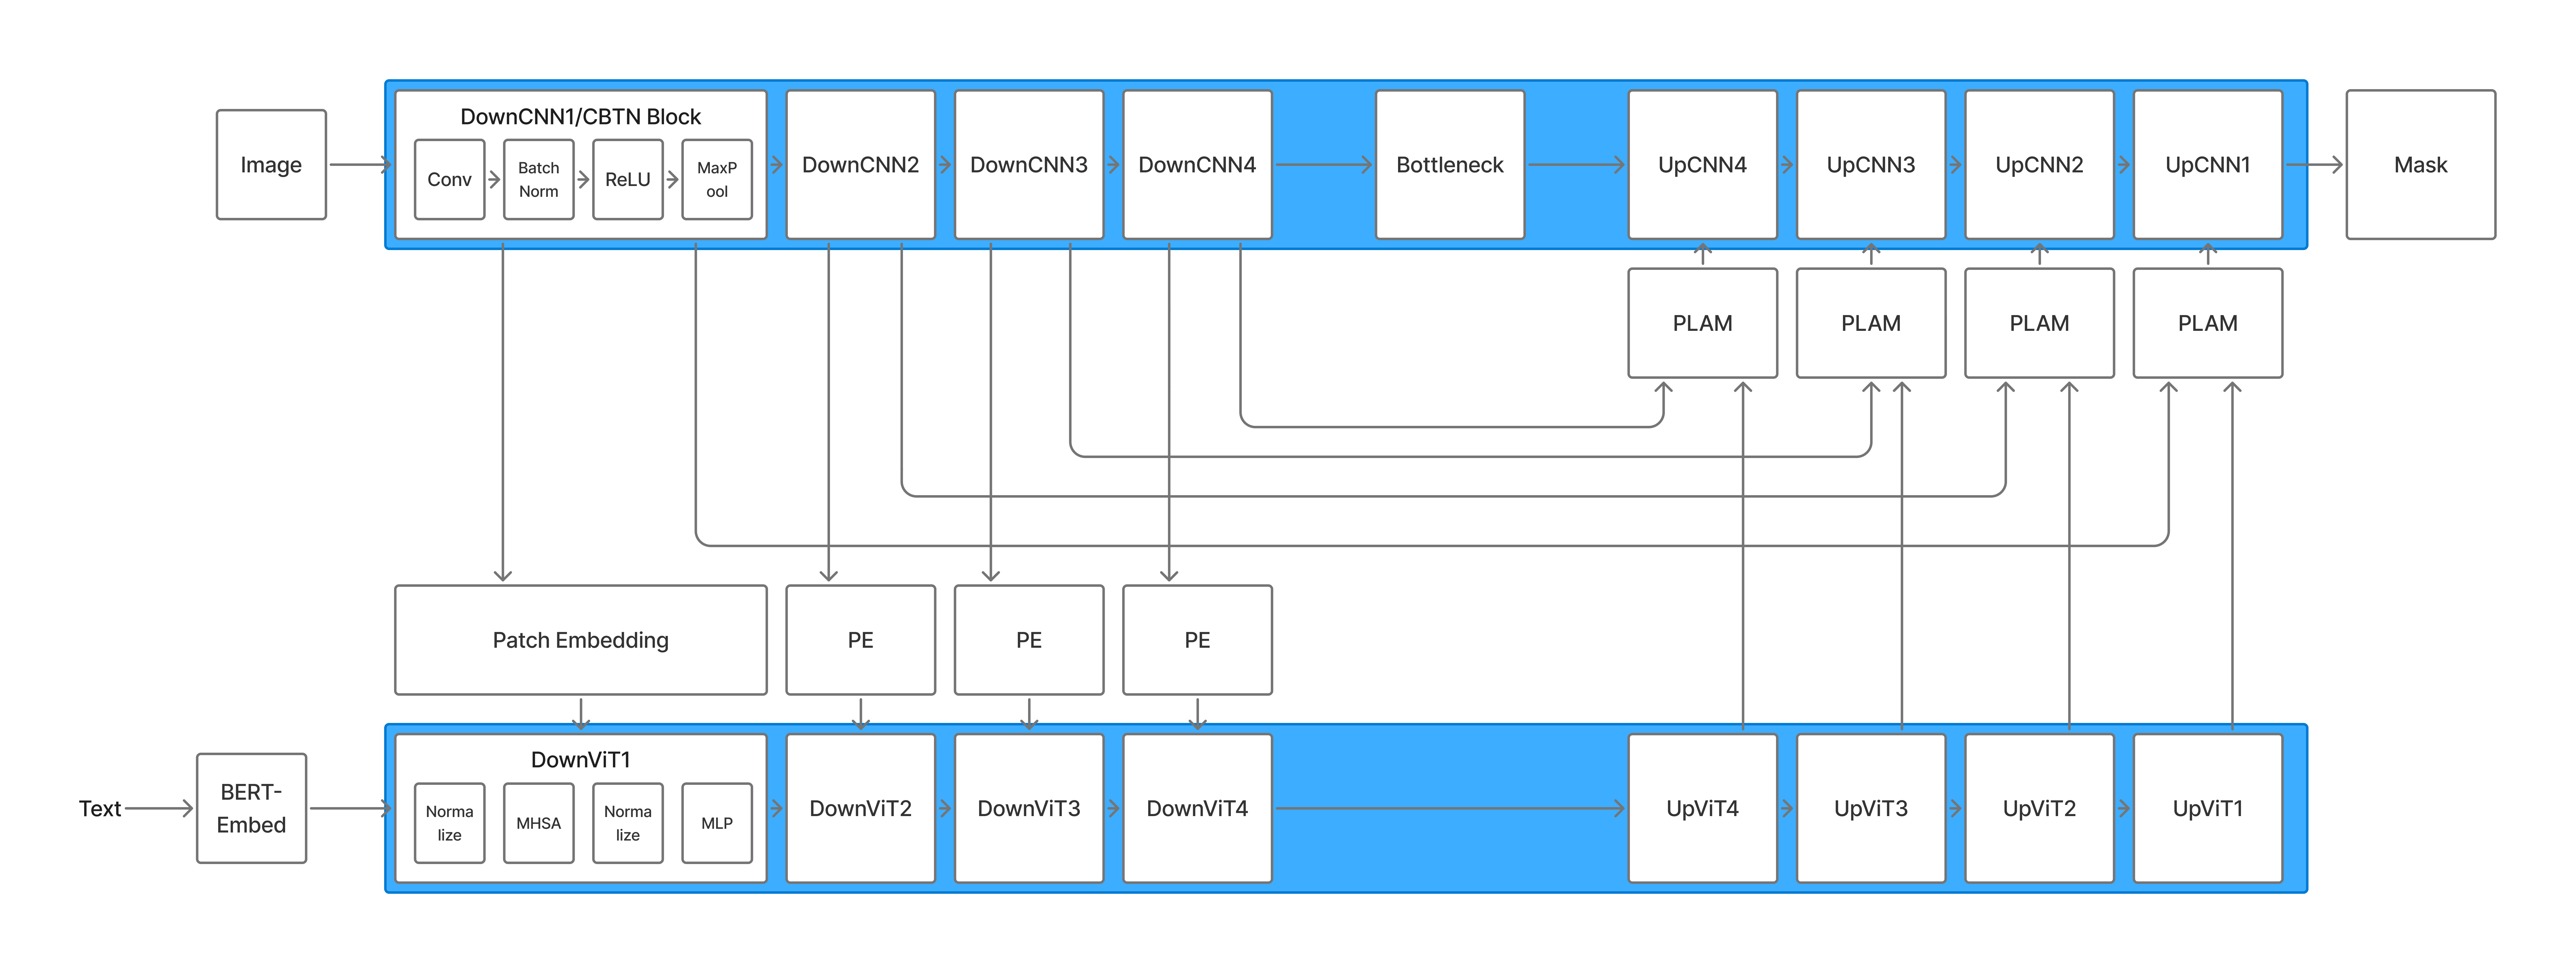
\includegraphics[width=\linewidth]{images/flatten-lvit.png}
    \caption{Kiến trúc mô hình LViT được trải thẳng}
\end{figure}

Mô hình LViT gồm 2 nhánh là: CNN và ViT. Trong đó nhánh ViT chịu trách nhiệm kết hợp thông tin văn bản và thông tin hình ảnh để trích xuất đặc trưng toàn cục theo kiến trúc Transformer, nhánh CNN chịu trách nhiệm trích xuất đặc trưng cục bộ trong hình ảnh. Sau đó, hai nhánh được kết hợp lại để tổng hợp đặc trưng cục bộ và toàn cục.

Nhánh CNN là nhánh chính, nhận đầu vào là một ảnh và đầu ra là bản đồ xác suất.
\begin{align*}
    D_i &= DownCNN_i = CTBN \\
        &= ReLU(BatchNorm_i(Conv_i(\cdot)))
\end{align*}
\[
    Y_{DownCNN, i+1} = MaxPool(D_i(Y_{DownCNN, i}))
\]
\[
    Y_{DownCNN, 0} = I
\]

\begin{figure}[H]
    
\includegraphics[width=0.5\linewidth]{images/cnn-branch.png}
    \caption{Nhánh CNN}
\end{figure}

Nhánh ViT là nhánh phụ, nhận đầu vào là đặc trưng ảnh của khối DownCNN đầu tiên cùng với đặc trưng văn bản từ lớp BERT-Embed của BERT\_12\_768\_12.

\begin{figure}[H]
    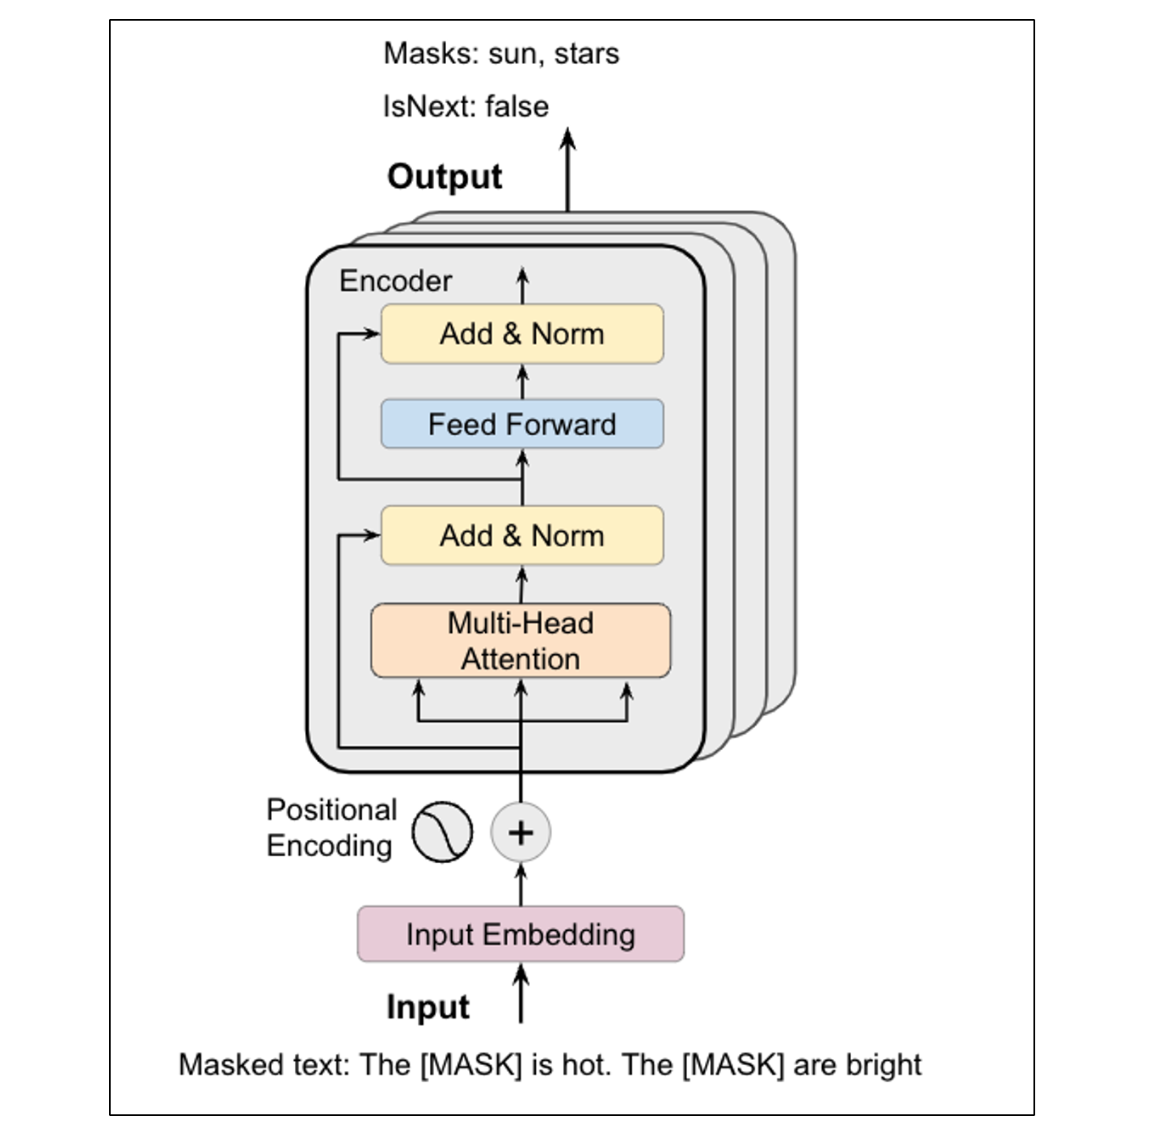
\includegraphics[width=0.5\linewidth]{images/bert.png}
    \caption{Sử dụng lớp Embedding đầu tiên của BERT}
\end{figure}

\begin{figure}[H]
    
\includegraphics[width=0.5\linewidth]{images/vit-branch.png}
    \caption{Nhánh ViT}
\end{figure}

    \[ViT(x) = ViT_2(ViT_1(x))\]
    \[x' = ViT_1(x) = MHSA(LN(x)) + x\]
    \[Y = ViT_2(x') = MLP(LN(x')) + x'\]
    \[x_{img, i} = PatchEmbedding(Y_{DownCNN, i})\]
    \[Y_{DownViT, 1} = ViT(x_{img, 1} + CTBN(x_{text}))\]
    \[Y_{DownViT, i+1} = ViT(Y_{DownViT, i} + x_{img, i + 1})\]

Mô-đun PLAM được thiết kế để bảo toàn đặc trưng cục bộ và tăng cường ngữ nghĩa trong đặc trưng văn bản.

Transformer thường có xu hướng thiên về việc học các đặc trưng toàn cục (global features) và bỏ qua chi tiết cục bộ. PLAM được thiết kế để bù đắp cho sự thiếu hụt này của cơ chế self-attention, giúp bảo tồn tối đa các đặc trưng cục bộ.

Phép cộng giúp hợp nhất các đặc trưng trên các kênh có ngữ nghĩa tương tự nhau nhằm tiết kiệm tính toán, trong khi phép nối giúp tích hợp thông tin trực quan và bảo tồn các đặc trưng gốc của từng phần. Sau khi nối, mô đun sử dụng cấu trúc MLP để căn chỉnh kích thước, đồng thời hòa trộn thêm các đặc trưng ngữ nghĩa từ văn bản vào hình ảnh.

\begin{figure}[H]
    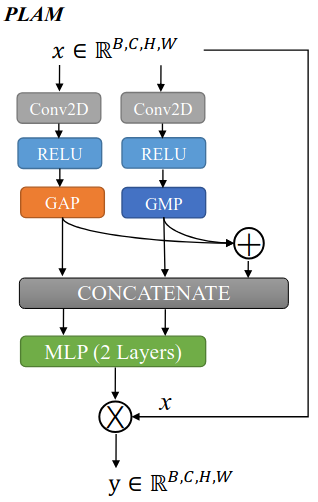
\includegraphics[width=0.5\linewidth]{images/plam.png}
    \caption{Mô-đun PLAM}
\end{figure}